%%simple header for compiling single bmad documentation tex files

\documentclass{book}

\usepackage{graphicx}
\usepackage{moreverb}
\usepackage{amsmath, amsthm, amssymb, amsbsy}
\usepackage{alltt}
\usepackage{rotating}
\usepackage[TABBOTCAP]{subfigure}
\usepackage{toc}
\usepackage{xspace}
%%\usepackage{makeidx}
\usepackage{index}
\usepackage{multirow}
\usepackage{booktabs}   % For table layouts
\usepackage{yhmath}     % For widehat

\usepackage[T1]{fontenc}   % so _, <, and > print correctly in text.
\usepackage[strings]{underscore}    % to use "_" in text
\usepackage[pdftex,colorlinks=true]{hyperref}   % Must be last package!

\newcommand{\extref}[1]{$\S$\ref*{#1}}   % No hyperlink. For external refs. \extref
\newcommand{\comma}{\> ,}
\newcommand{\period}{\> .}
\newcommand{\wt}{\widetilde}
\newcommand{\grv}{\textasciigrave}
\newcommand{\hyperbf}[1]{\textbf{\hyperpage{#1}}}
\newcommand{\Ss}{\(^*\)}
\newcommand{\Dd}{\(^\dagger\)}

\newcommand{\AND}{&& \hskip -17pt\relax}
\newcommand{\CR}{\\}
\newcommand{\CRNO}{\nonumber \\}
\newcommand{\dstyle}{\displaystyle}

\newcommand{\Begineq}{\begin{equation}}
\newcommand{\Endeq}{\end{equation}}
\newcommand{\NoPrint}[1]{}

\newcommand{\pow}[1]{\cdot 10^{#1}}
\newcommand{\Bf}[1]{{\bf #1}}
\newcommand{\bfr}{\Bf r}

\newcommand{\bmad}{{\sl Bmad}\xspace}
\newcommand{\tao}{{\sl Tao}\xspace}
\newcommand{\mad}{{\sl MAD}\xspace}
\newcommand{\cesr}{{\sl CESR}\xspace}

\newcommand{\sref}[1]{\S\ref{#1}}
\newcommand{\Sref}[1]{Sec.~\sref{#1}}
\newcommand{\cref}[1]{Chapter~\ref{#1}}

\newcommand{\Newline}{\hfil \\ \relax}

\newcommand{\eq}[1]{{(\protect\ref{#1})}}
\newcommand{\Eq}[1]{{Eq.~(\protect\ref{#1})}}
\newcommand{\Eqs}[1]{{Eqs.~(\protect\ref{#1})}}

\newcommand{\vn}{\ttcmd}           % For variable names
\newcommand{\vni}{\ttcmdindx}
\newcommand{\cs}{\ttcmd}           % For code source
\newcommand{\cmd}{\ttcmd}          % For Unix commands
\newcommand{\rn}{\ttcmd}           % For Routine names
\newcommand{\tn}{\ttcmd}           % For Type (structure) names
\newcommand{\bn}[1]{{\bf #1}}       
\newcommand{\toffset}{\vskip 0.01in}
\newcommand{\rot}[1]{\begin{rotate}{-45}#1\end{rotate}}

\newcommand{\data}{{\mbox{data}}}
\newcommand{\reference}{{\mbox{ref}}}
\newcommand{\model}{{\mbox{model}}}
\newcommand{\base}{{\mbox{base}}}
\newcommand{\design}{{\mbox{design}}}
\newcommand{\meas}{{\mbox{meas}}}
\newcommand{\var}{{\mbox{var}}}

\newcommand\ttcmd{\begingroup\catcode`\_=11 \catcode`\%=11 \dottcmd}
\newcommand\dottcmd[1]{\texttt{#1}\endgroup}

\newcommand\ttcmdindx{\begingroup\catcode`\_=11 \catcode`\%=11 \dottcmdindx}
\newcommand\dottcmdindx[1]{\texttt{#1}\endgroup\index{#1}}

\newcommand{\St}{$^{st}$\xspace}
\newcommand{\Nd}{$^{nd}$\xspace}
\newcommand{\Th}{$^{th}$\xspace}
\newcommand{\B}{$\backslash$}
\newcommand{\W}{$^\wedge$}

\newcommand{\cbar}[1]{\overline C_{#1}}

\newlength{\dPar}
\setlength{\dPar}{1.5ex}

\newenvironment{example}
  {\vspace{-3.0ex} \begin{alltt}}
  {\end{alltt} \vspace{-2.5ex}}

\newcommand\Strut{\rule[-2ex]{0mm}{6ex}}

\newenvironment{Itemize}
  {\begin{list}{$\bullet$}
    {\addtolength{\topsep}{-1.5ex} 
     \addtolength{\itemsep}{-1ex}
    }
  }
  {\end{list} \vspace*{1ex}}

\newcommand{\Section}[1]{\section{#1}\indent\vspace{-3ex}}

\newcommand{\SECTION}[1]{\section*{#1}\indent\vspace{-3ex}}

% From pg 64 of The LaTex Companion.

\newenvironment{ventry}[1]
  {\begin{list}{}
    {\renewcommand{\makelabel}[1]{\textsf{##1}\hfil}
     \settowidth{\labelwidth}{\textsf{#1}}
     \addtolength{\itemsep}{-1.5ex}
     \addtolength{\topsep}{-1.0ex} 
     \setlength{\leftmargin}{5em}
    }
  }
  {\end{list}}


\setlength{\textwidth}{6.25in}
\setlength{\hoffset}{0.0in}
\setlength{\oddsidemargin}{0.25in}
\setlength{\evensidemargin}{0.0in}
\setlength{\textheight}{8.5in}
\setlength{\topmargin}{0in}

\makeindex
\newindex{routine}{rdx}{rnd}{Routine Index}

\begin{document}



\chapter{Tracking and Transfer Maps}
\label{c:tracking}
\index{tracking}

\index{macroparticles!tracking}
\index{tracking!Macroparticles}
\bmad has routines for tracking two types of objects called
``\vn{particles}'' and ``\vn{macroparticles}''. \vn{Particles} are
characterized by a six-vector representing the particle's phase space
coordinates and a pair of complex numbers characterizing the
particle's spin.  A macroparticle is like a particle with the
addition of a $6\times 6$ ``sigma'' matrix characterizing the size of
the macroparticle.

Macroparticle tracking was implemented in \bmad in order to simulate particle bunches.
The idea was that far fewer macroparticles than particles would 
be needed to characterize a bunch. In practice, it was found that the complexity 
of handling the macroparticle sigma matrix more than offset the reduction in the
number of particles needed. Hence, while the basic macroparticle tracking 
routines still exist, macroparticle tracking is not currently maintained
and the use of this code is discouraged. However macroparticle tracking could be revived
in the future if there is a demonstated need for it.

\index{beam}\index{bunch}
Particle tracking can be divided into ``single particle'' tracking and ``beam''
tracking. Single particle tracking is simply tracking a single particle.
Beam tracking is tracking an ensable of particles divided up into a number of bunches
that make up a ``beam''. Both types particle tracking are covered in this
chapter.

%----------------------------------------------------------------
\section{The coord_struct}
\index{coord_struct}

\index{spin}
\index{phase space coordinates}
The \vn{coord_struct} holds the coordinates of a particle at a given
longitudinal position in the lattice. The definition of the
\vn{coord_struct} is
\begin{example}
  type coord_struct
    real(rp) vec(6)       ! (x, px, y, py, z, pz)
    complex(rp) spin(2)   ! particle spin in spinor notation
    real(rp) e_field_x    ! Photon field/sqrt(area), x-axis component
    real(rp) e_field_y    ! Photon field/sqrt(area), y-axis component
    real(rp) phase_x      ! Photon phase, x-axis component
    real(rp) phase_y      ! Photon phase, y-axis component
    real(rp) s            ! Longitudinal position 
    real(rp) t            ! Time
  end type
\end{example}
The \vn{%vec(6)} array defines the phase space coordinants
(\sref{s:phase.space}) and spin (\sref{s:spin.dyn}). The \vn{%s}
component gives the absolute s-position of the particle and \vn{%t}
gives the absolute time.

The \vn{%e_field_x} and \vn{%e_field_y} components are for photon
tracking and are in units of field/sqrt(cross-section-area). That is,
the square of these units is an intensity. It is up to individual
programs to define an overall scaling factor for the intensity if
desired.

When associated with a lattice element, a \vn{coord_struct} variable
gives a particle's position at the exit end of the element.  To get an
orbit through a lattice branch (\sref{s:lat.struct}), that is, the
particle position at every element in the branch, an array of
\vn{coord_struct}s is needed. Since the number of elements in the
lattice is not known in advance, the array must be declared to be
allocatable. The lower bound of the array must be set to zero to match
a \vn{lat%branch(i)%ele(:)} array.  The upper bound should be the
upper bound of the \vn{%branch(i)%ele(:)} array.  The routine
\Hyperref{r:reallocate.coord}{reallocate_coord} will allocate an array
of \vn{coord_struct}s:
\begin{example}
  type (coord_struct), allocatable :: orbit(:)
  type (lat_struct) lat
  ...
  call reallocate_coord (orbit, lat%branch(i)%n_ele_max)
  orbit(0)%vec = [0.01, 0.2, 0.3, 0.4, 0.0, 0.0] ! init
  ...
  deallocate(orbit) ! Needed if orbit is a local var
\end{example}
The deallocation at the end of this example is needed when the
\vn{coord_struct} array is defined locally (not passed as an argument)
in a subroutine or function. Alternatively, the \vn{save} attribute
can be used so that the array stays around until the next time the
routine is called
\begin{example}
  type (coord_struct), allocatable, save :: orb(:) 
\end{example}
Saving the \vn{coord_stuct} is faster but leaves memory tied up. Note
that in the main program, the \vn{save} attribute is not permitted and
the deallocation is not necessary.  If a \vn{coord_struct} array is
passed to a routine, the routine must explicitly set the lower bound
to zero if the array is not declared as allocatable:
\begin{example}
  subroutine my_routine (orbit1, orbit2)
    use bmad
    implicit none
    type (coord_struct), allocatable :: orbit1(:)  ! OK
    type (coord_struct) orbit2(0:)                 ! Also OK
    ...
\end{example}
Declaring the array allocatable is manditory if the array is to be resized
or the array is passed to a routine that declares it allocatable.

\index{coord_array_struct}
For an entire lattice, the \vn{coord_array_struct} can be used to define an array
of \vn{coord_array} arrays:
\begin{example}
  type coord_array_struct
    type (coord_struct), allocatable :: orb(:)
  end type
\end{example}
The routine \Hyperref{r:reallocate.coord.array}{reallocate_coord_array} will allocate an
\vn{coord_array_struct} instance
\begin{example}
  type (coord_array_struct), allocatable :: all_orbit(:)
  type (lat_struct) lat
  ...
  call reallocate_coord_array (all_orbit, lat)
  ...
  deallocate(all_orbit) ! Needed if all_orbit is a local var
\end{example}

%----------------------------------------------------------------
\section{Tracking Through a Lattice Element}
\label{s:ele.track}

The ``entrance'' and ``exit'' ends of a lattice element are, by definition,
where the physical ends of the element would be if there were no
offsets. In particular, if an element has a finite \vn{s_offset}
(\sref{s:ele.offset}), the physical ends will be displaced from
the entrance and exit ends. Thus, the position \vn{ds} of a particle with
respect to the physical beginning of the element is
\begin{example}
  ds = coord%s - (ele%s + ele%value(s_offset_tot\$) - ele%value(l\$))
\end{example}

When tracking through a lattice element that has finite offsets, the
\Hyperref{r:offset.particle}{offset_particle} routine can be called to
convert between laboratory and element coordinates
(\sref{s:misalign.track}). In particular, if there is a finite
\vn{s_offset}, the \vn{offset_particle} routine will insert drifts
just before and just after the tracking of the body of the element so
that the particle begins at the entrance face and ends at the exit
face independent of the actual physical placement of the element.

%----------------------------------------------------------------
\section{Closed Orbit and Particle Tracking}

\index{closed orbit}
For a circular lattice the closed orbit may be calculated using
\vn{closed_orbit_calc}. By default this routine will track in the
forward direction which is acceptable unless the particle you are
trying to simulate is traveling in the reverse direction and there is
radiation damping on. In this case you must tell
\vn{closed_orbit_calc} to do backward tracking. This routine works by
iteratively converging on the closed orbit using the 1--turn matrix to
calculate the next guess. On rare occasions if the nonlinearities are
strong enough, this can fail to converge. An alternative routine is
\vn{closed_orbit_from_tracking} which tries to do things in a more
robust way but with a large speed penalty.

The routine \Hyperref{r:track.all}{track_all} tracks thourgh a given branch of the
lattice.  Multi-turn tracking over a branch is then simply a matter of
setting the coordinates at the beginning zeroth element equal to the
last tracked element within a loop:
\begin{example}
  type (lat_struct) lat             ! lattice to track through
  type (coord_struct), allocatable :: orbit(:)
  ...
  call reallocate_coord (orbit, lat%branch(1)%n_ele_max)
  orbit(0)%vec = [0.01, 0.2, 0.3, 0.4, 0.0, 0.0] ! init
  do i = 1, n_turns
    call track_all (lat, orbit, 1)
    orbit(0) = orbit(lat%branch(1)%n_ele_track)
  end do
\end{example}
Often times it is only the root branch, \vn{branch(0)}, that is to be tracked.
In this case, the above reduces to
\begin{example}
  type (lat_struct) lat             ! lattice to track through
  type (coord_struct), allocatable :: orbit(:)
  ...
  call reallocate_coord (orbit, lat%n_ele_max)
  orbit(0)%vec = [0.01, 0.2, 0.3, 0.4, 0.0, 0.0] ! init
  do i = 1, n_turns
    call track_all (lat, orbit)
    orbit(0) = orbit(lat%n_ele_track)
  end do
\end{example}

The routine \Hyperref{r:track1}{track1} is the routine that tracks through one
element in the lattice. The routine \Hyperref{r:track.all}{track_all} calls \vn{track1}
in a loop over all elements to track through the entire
lattice. Alternatively the routine \Hyperref{r:track.many}{track_many} can be used to
track through a selective number of elements or to track backwards
(See \sref{s:reverse.track}). The routines used for tracking
and closed orbit calculations are listed in Section \sref{r:track}.

\index{lat_param_struct!lost}
\index{lat_param_struct!ix_lost}
\index{lat_param_struct!plane_lost_at}
\index{lat_param_struct!end_lost_at}
\index{tracking!example}
The \vn{track_all} routine serves as a good example of how tracking
works. \vn{track_all} tracks a particle through a lattice from
beginning to end. Its code, condensed slightly, is shown in
Figure~\ref{f:track.all}.  The \vn{reallocate_coord} call (line~13) is
done in case the number of elements in the lattice has changed. The
call to \vn{track1} (line~18) tracks through one element from the exit
end of the $n-1$\St\ element to the exit end of the $n$\Th
particle. \vn{lat%param%lost} is a logical that signals the
calling routine whether a particle has been lost.  This generally
happens when the particle's position is larger then the aperture. When
a particle is lost \vn{lat%param%ix_lost} is used to record in
what element the loss occurred.

\begin{figure}[htb]
\begin{centering}
\small
\begin{listing}{1}
  subroutine track_all (lat, orbit)
    use bmad_struct
    use bmad_interface
    implicit none
    type (lat_struct)  lat
    type (coord_struct), allocatable :: orbit(:)
    integer n

  ! Init

    lat%param%lost = .false.
    if (size(orbit) < lat%n_ele_max+1) &
                    call reallocate_coord (orbit, lat%n_ele_max)

  ! Track through the elements and check for lost particles.

    do n = 1, lat%n_ele_track
      call track1 (orbit(n-1), lat%ele(n), lat%param, orbit(n))
      if (lat%param%lost) then
        lat%param%ix_lost = n
        return
      endif
    enddo
  end subroutine
\end{listing}
\label{f:track.all}
\caption{Condensed track_all code.}
\end{centering}
\end{figure}

%----------------------------------------------------------------
\section{Partial Tracking through elements}
\label{s:tracking.partial}
\index{tracking!partial}

There are two routines for tracking partially through an element:
\begin{example}
  \Hyperref{r:twiss.and.track.at.s}{twiss_and_track_at_s} (lat, s, ele, orb, orb_at_s, ix_branch, err, use_saved_data)
  \Hyperref{r:twiss.and.track.intra.ele}{twiss_and_track_intra_ele}  (ele, param, l_start, l_end, track_entrance,
                   track_exit, orbit_start, orbit_end, ele_start, ele_end, err)

\end{example}
Both routines make use of element ``slices'' (\sref{s:ele.lat}) which
are elements that represent some sub-section of an element. The
routine \Hyperref{r:create.element.slice}{create_element_slice} can be used to create such slices.

%----------------------------------------------------------------
\section{Apertures}
\label{s:tracking.apertures}
\index{tracking!apertures}

\index{ele_struct!\%aperture_type}
The routine \Hyperref{r:check.aperture.limit}{check_aperture_limit}
checks the aperture at a given element. The \vn{ele%aperture_type}
component determines the type of aperture. Possible values for
\vn{ele%aperture_type} are
\begin{example}
  rectangular$
  elliptical$
  custom$
\end{example} %$
With \vn{custom\$}, a program needs to be linked with a custom version
of
\Hyperref{r:check.aperture.limit.custom}{check_aperture_limit_custom}.

\index{lat_param_struct!aperture_limit_on}
\index{bmad_common_struct!max_aperture_limit}
The logical \vn{lat%param%aperture_limit_on} determines if element
apertures (See \sref{s:limit}) are used to determine if a
particle has been lost in tracking.  The default
\vn{lat%param%aperture_limit_on} is True.  Even if this is False
there is a ``hard'' aperture limit set by
\vn{bmad_com%max_aperture_limit}. This hard limit is used to prevent
floating point overflows. The default hard aperture limit is 1000
meters. Additionally, even if a particle is within the hard limit,
some routines will mark a particle as lost if the tracking calculation
will result in an overflow.

\index{lat_param_struct!end_lost_at}
\index{lat_param_struct!lost}
\index{lat_param_struct!ix_lost}
\index{entrance_end}
\index{exit_end}
\vn{lat%param%lost} is the logical to check to see if a particle has
been lost. \vn{lat%param%ix_lost} is set by \vn{track_all} and gives
the index of the element at which a particle is lost.
\vn{%param%end_lost_at} gives which end the particle was lost at. 
The possible values for \vn{lat%param%end_lost_at} are:
\begin{example}
  entrance_end\$
  exit_end\$
\end{example}
When tracking forward, if a particle is lost at the exit end of an
element then the place where the orbit was outside the aperture is at
\vn{orbit(ix)} where \vn{ix} is the index of the element where the
particle is lost (given by \vn{lat%param%ix_lost}). If the
particle is lost at the entrance end then the appropriate index is one
less (remember that \vn{orbit(i)} is the orbit at the exit end of an
element). 

To tell how a particle is lost, check the \vn{lat%param%plane_lost_at}
parameter. Possible values for this are:
\begin{example}
  x_plane\$
  y_plane\$
  z_plane\$
\end{example}
\vn{x_plane\$} and \vn{y_plane\$} indicate that the particle was lost
either horizontally, or vertically. \vn{z_plane\$} indicates that the
particle was turned around in an \vn{lcavity} element. That is, the 
cavity was deaccelerating the particle and the particle did not not have
enough energy going into the cavity to make it to the exit.

%======================FIGURE===============================
\begin{figure}[tb]
\centering
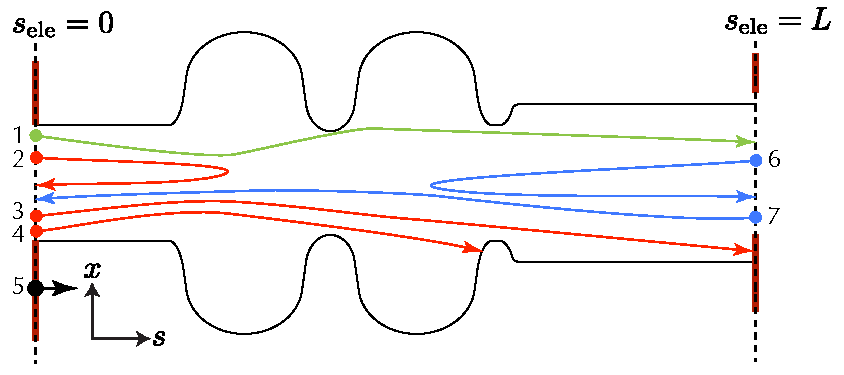
\includegraphics[width=\textwidth]{tracking-apertures}
\caption[Example trajectories in the element coordinate system.]{
Example trajectories in the element coordinate system. 
Note that the wall and apertures are aligned at $s_{\rm ele} =0$, 
but offset at $s_{\rm ele} = L.$}
\label{fg:tracking-apertures}
\end{figure}
%===========================================================

%======================TABLE=============================
\begin{table}[tb]
\caption[Possible aperture flags set when tracking an individual element.]{
Possible aperture flags set when tracking an individual element. 
Trajectories are labeled as in Fig.~\ref{fg:tracking-apertures}}
\begin{tabular*}{\columnwidth}{@{\extracolsep{\fill}}lrrr}
\toprule
 Example particle trajectory & \vn{lost} & \vn{plane_lost_at} & \vn{end_lost_at}\\ 
 \midrule
1: Forward  					& F &  \vn{z_plane\$} & \vn{exit_end\$}  \\
2: Forward kicked backwards	& T &  \vn{z_plane\$} & \vn{live_reversed\$} \\
3: Hits exit aperture 		& T &  \vn{x_plane\$} & \vn{exit_end\$} \\
4: Hits interior wall 		& T &  \vn{x_plane\$} & \vn{between_ends\$} \\
5: Enters outside aperture 	& T &  \vn{x_plane\$} & \vn{entrance_end\$} \\
6: Backwards 				& T &  \vn{z_plane\$} & \vn{live_reversed\$} \\
7: Backwards kicked forward & F &  \vn{z_plane\$} & \vn{exit_end\$} \\
\bottomrule
\end{tabular*}
\label{tb:tracking-apertures}
\end{table}
%=====================TABLE===============================

%----------------------------------------------------------------
\section {Tracking Methods}

\index{ele_struct!\%tracking_method}
For each element the method of tracking may be set either via the
input lattice file (see \sref{s:tkm}) or directly in the
program by setting the \vn{%tracking_method} attribute of an element
\begin{verbatim}
  type (ele_struct) ele
  ...
  ele%tracking_method = boris$  ! for boris tracking
  print *, 'Tracking_method: ', calc_method_name(ele%tracking_method)
\end{verbatim}
To form the corresponding parameter to a given tracking method just
put ``\$'' after the name. For example, the \vn{bmad_standard}
tracking method is specified by the \vn{bmad_standard\$} parameter. To
convert the integer \vn{%tracking_method} value to a string suitable
for printing, use the \vn{tracking_method_name} array.

\index{ele_struct!\%mat6}\index{linear}
It should be noted that except for \vn{linear} tracking, none of the
\bmad tracking routines make use of the \vn{ele%mat6} transfer
matrix. The reverse, however, is not true.  The transfer matrix
routines (\vn{lat_make_mat6}, etc.)  will do tracking.


\index{synchrotron radiation!calculating}
\bmad simulates radiation damping and excitation by applying a kick
just before and after each element. 

%----------------------------------------------------------------
\section{Taylor Maps}
\label{s:taylor.track}
\index{taylor Map}

A list of routines for manipulating Taylor maps is given
in~\sref{r:taylor}. The order of the Taylor maps is set in the lattice
file using the \vn{parameter} statement (\sref{s:param}). In a program
this can be overridden using the routine \Hyperref{r:set.taylor.order}{set_taylor_order}. The
routine \Hyperref{r:taylor.coef}{taylor_coef} can be used to get the coefficient of any
given term.

\index{symp_lie_Bmad}
\index{symp_lie_PTC}
\index{symp_map}
\index{taylor}
\index{taylor!deallocating}
Transfer Taylor maps for an element are generated as needed when the
\vn{ele%tracking_method} or \vn{ele%mat6_calc_method} is set to
\vn{Symp_Lie_Bmad}, \vn{Symp_Lie_PTC}, \vn{Symp_Map}, or
\vn{Taylor}. Since generating a map can take an appreciable time,
\bmad follows the rule that once generated, these maps are never
regenerated unless an element attribute is changed.  To generate a
Taylor map within an element irregardless of the
\vn{ele%tracking_method} or \vn{ele%mat6_calc_method} settings use the
routine \Hyperref{r:ele.to.taylor}{ele_to_taylor}. This routine will kill any old Taylor map
before making any new one. To kill a Taylor map (which frees up the
memory it takes up) use the routine \Hyperref{r:kill.taylor}{kill_taylor}.

To test whether a \vn{taylor_struct} variable has an associated Taylor
map. That is, to test whether memory has been allocated for the map,
use the Fortran associated function:
\begin{example}
  type (bmad_taylor) taylor(6)
  ...
  if (associated(taylor(1)%term)) then  ! If has a map ...
    ...
\end{example}

To concatenate the Taylor maps in a set of elements the routine
\Hyperref{r:concat.taylor}{concat_taylor} can be used
\begin{example}
  type (lat_struct) lat          ! lattice
  type (taylor_struct) taylor(6)  ! taylor map
  ...
  call taylor_make_unit (taylor)  ! Make a unit map
  do i = i1+1, i2
    call concat_taylor (taylor, lat%ele(i)%taylor, taylor)
  enddo
\end{example}
The above example forms the transfer Taylor map starting at the end of
element \vn{i1} to the end of element \vn{i2}. Note: This example
assumes that all the elements have a Taylor map. The problem with
concatenating maps is that if there is a constant term in the map
``feed down'' can make the result inaccurate (\sref{s:taylor.phys}. To
get around this one can ``track'' a taylor map through an element
using symplectic integration.
\begin{example}
  type (lat_struct) lat          ! lattice
  type (taylor_struct) taylor(6)  ! taylor map
  ...
  call taylor_make_unit (taylor)  ! Make a unit map
  do i = i1+1, i2
    call call taylor_propagate1 (taylor, lat%ele(i), lat%param)
  enddo
\end{example}
\index{ds_step}
\index{integrator_order}
Symplectic integration is typically much slower than concatenation.
The width of an integration step is given by \vn{%ele%value(ds_step\$}.
The attribute \vn{%ele%value(num_steps\$)}, which gives the number
of integration steps, is a dependent variable 
(\sref{s:depend}) and should not be set directly.
The order of the integrator (\sref{s:taylor.phys})
is given by \vn{%ele%integrator_order}. 
PTC (\sref{c:etienne}) currently implements integrators of order 2, 4, or 6.

%----------------------------------------------------------------
\section{Reverse Tracking}
\label{s:reverse.track}
\index{tracking!reverse}

There are two ways to do reverse tracking in which the particle goes
in the direction of decreasing \vn{s}. The first way is to use the
\Hyperref{r:track.many}{track_many} routine. See the \vn{track_many}
routine for more details. The advantage of using \vn{track_many} is
that it is simple. The disadvantage is that it can slow things down
some since each element goes through a reversal process every time it
is tracked through. If a program is doing a lot of tracking the other
option is to form a reversed lattice with the elements in the reverse
order and track through that. The routine
\Hyperref{r:lat.reverse}{lat_reverse} will do this. One must be
somewhat careful since the reversed lattice uses a reversed coordinate
system. The transformation between the reversed and unreversed
lattices is
\Begineq
  (x, p_x, y, p_y, z, p_z) -> (x, -p_x, -y, p_y, -z, p_z)
\Endeq
See the \vn{lat_reverse} routine for more details.

Generally tracking backwards is simply the reverse of tracking
forwards (time reversal symmetry). That is, if you start at some
place, track forward for some distance and then track back to the
starting place the ending orbit will be equal to the starting
orbit. However, it should always be kept in mind that radiation
damping or excitation breaks this symmetry.

%----------------------------------------------------------------
\section{Particle Distribution Tracking}
\label{s:part.track}
\index{tracking!particle distributions}

Initializing a distribution of particles to conform to some initial set of
Twiss parameters and emittances can be done using the routine
\Hyperref{r:init.beam.distribution}{init_beam_distribution}. 

%----------------------------------------------------------------
\section{Spin Tracking}
\label{s:spin.track}
\index{tracking!spin}

See Section~\sref{s:spin.methods} for a list of spin tracking methods
available. To turn spin tracking on, use the
\vn{bmad_com%spin_tracking_on} flag. After properly initializing the
spin in the \vn{coord_struct}, calls to \vn{track1} will track both
the particle orbit and the spin.

%-----------------------------------------------------------------------------
\section{Custom Field Calculations}
\label{s:custom.field}
\index{fields (electric and magnetic)!custom calculation} 
\index{ele_struct!\%field_calc}

\index{runge_kutta}\index{boris}\index{ele_struct!\%field_calc}
\Hyperref{r:em.field.custom}{em_field_custom}
Custom Electric and Magnetic field calculations are used with
\vn{runge_kutta} and \vn{boris} tracking (See \sref{s:integ}).  To
implement custom field calculations the \vn{ele%field_calc} component
of an element must be set to \vn{custom\$}. This can be done either
through the lattice input file or within a program. Additionally a
routine \vn{em_field_custom} must be linked with any program using the
custom calculations.

%\end{document}